\section{Memoria}

L'architettura pensata da Von Neumann richiede una grande quantità di memoria rapida dove salvare tutti i dati dei programmi, questo non è però economicamente possibile.

\spacer
La memoria principale dei sistemi moderni costituita da \textbf{DRAM} (\textit{Dynamic Random Access Memory}) è molto più lenta della CPU limitandone così le prestazioni.

Le memorie con prestazioni comparabili a quelle della CPU sono le \textbf{SRAM} (\textit{Static Random Access Memory}) che sono però troppo costose e quindi possono essere utilizzate solo in quantità limitata.

\spacer
Per questo motivo si costruisce una piramide attorno alla memoria principale, con cache più rapide e piccole al di sopra e dischi lenti, ma estremamente capienti, al di sotto.

\begin{figure}[H]
    \centering
    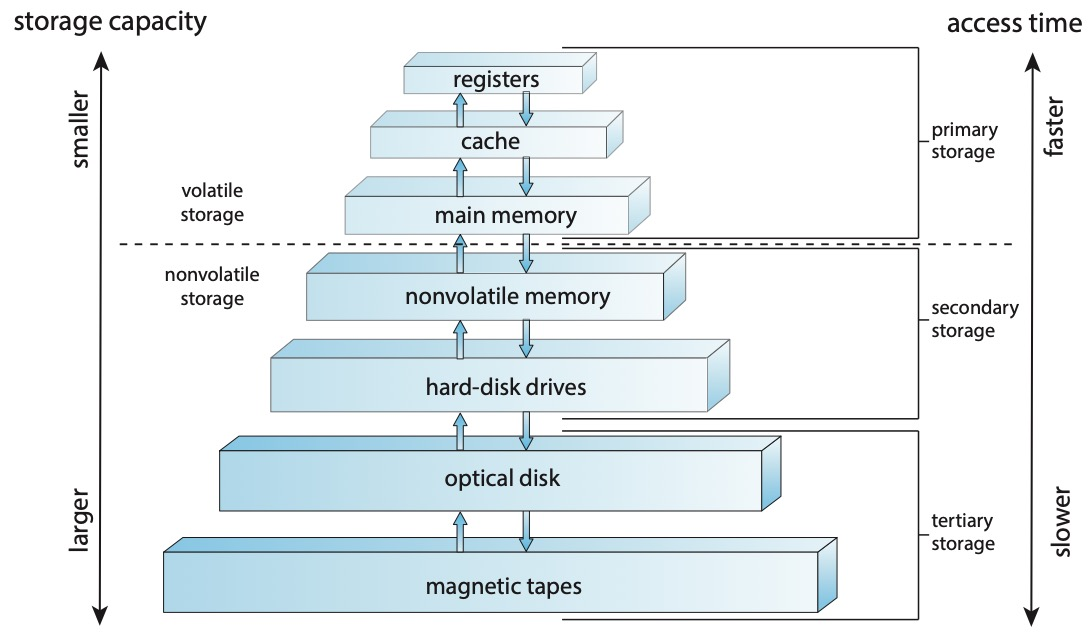
\includegraphics[width=0.48\linewidth]{assets/storage-hierarchy.jpg}
\end{figure}

\subsection{Cache}

La cache si inserisce tra il processore e la memoria principale, quando la CPU richiede un valore esso viene prima cercato nella cache:
\spacer
\begin{sitemize}
    \item \textbf{cache hit:} Il valore viene trovato e può essere restituito alla CPU rapidamente.
    \item \textbf{cache miss:} Il valore non viene trovato, quindi sarà necessario attendere la DRAM.

    Dopo aver recuperato il valore esso, e i valori adiacenti, vengono salvati nella cache, applicando una politica di rimpiazzo se la cache è piena.
\end{sitemize}

\spacer
L'obiettivo è quello di rendere il più grande possibile la percentuale di cache hit sul totale delle richieste.

Per ottenere questo è particolarmente importante sviluppare una \textbf{politica di rimpiazzo} efficace, due principi efficaci a questo scopo:

\spacer
\begin{sitemize}
    \item \textbf{Località spaziale:} È probabile che la CPU debba accedere alle celle adiacenti, come nel caso della lettura di un vettore. È quindi conveniente copiare non solo la cella, ma un intero blocco di memoria RAM.
    \item \textbf{Località temporale:} È più probabile che venga richiesto un dato che è stato chiesto poco prima.
\end{sitemize}

\subsubsection*{Livelli di Cache}
Spesso per ottimizzare i tradeoff della cache essa viene organizzata in livelli (L1, L2, ...) dove più basso è il livello più la cache è piccola e veloce.
Questo viene fatto perché una cache L1 è molto più costosa di una L2 e così via.


Normalmente possiamo dire che la cache di livello $i + 1$ contiene tutti i dati della cache di livello $i$

\begin{note}
    Le prestazioni della cache sono particolarmente importanti per prestazioni dell'intero sistema, se viene progettata in modo corretto può garantire che una percentuale dall'80\% al 99\% degli accessi si limiti ad essa, senza andare alla memoria RAM.
\end{note}

\subsubsection{Esempio}
Una microarchittetura con 3 livelli di cache può essere sturtturata nel seguente modo:

\spacer
\begin{sitemize}
    \item Una cache L1 interna alla CPU, che contiene una parte per le istruzioni, L1-I (16 Kbyte) e una parte per i dati L1-D (64 Kbyte).
    \item Una cache L2, esterna alla CPU, ma contenuta comunque nel package. Di dimensioni maggiori (512 Kb - 1 Mb)
    \item Una cache L3, presente sulla motherboard
\end{sitemize}

\spacer
Le cache L1 e L2, interne al package, hanno un bus riservato, aumentando così le prestazioni.

\begin{figure}[H]
    \centering
    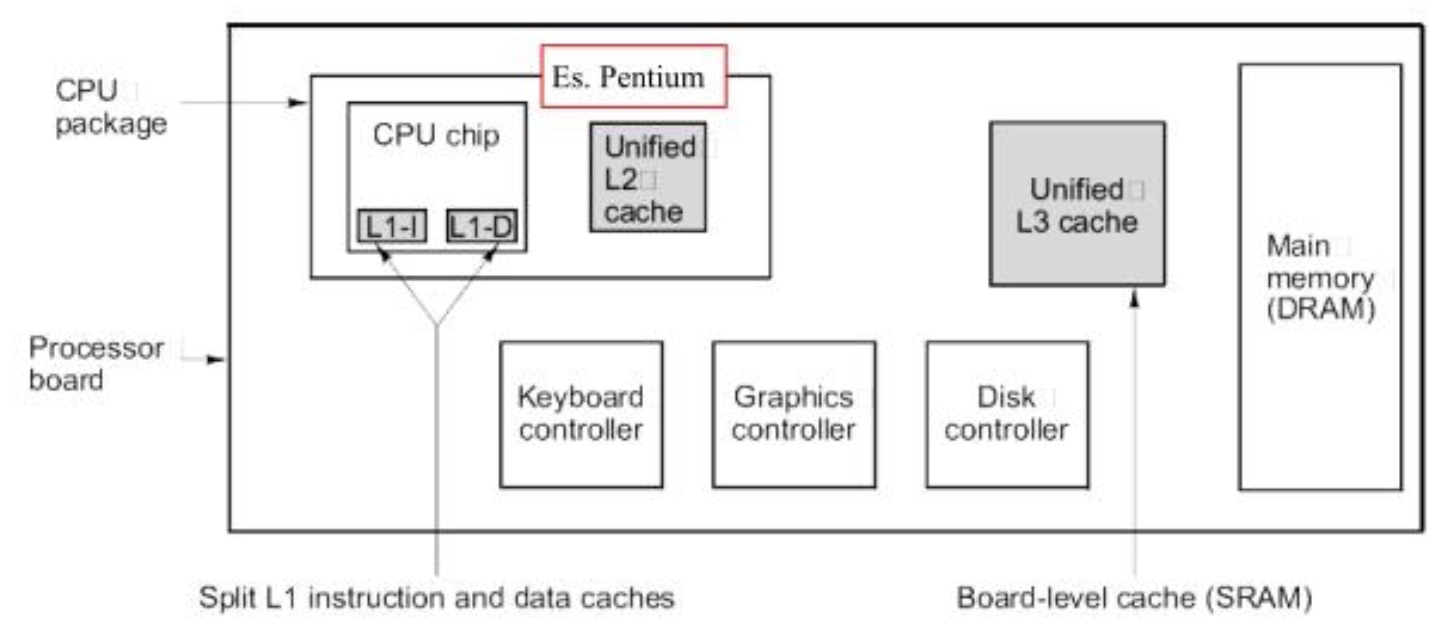
\includegraphics[width=0.5\linewidth]{assets/pentium-cache-architecture.jpeg}
\end{figure}

